\section{Portable}
\label{ch:portable}

1.	The Stirling engine is a battery charger with hot water output. The only task is to produce hot water and to charge the battery during operation. I included the basic flow chart section for this. 

2.	The Inverter task is to select on-grid or off-grid mode and to control voltage, frequency etc. The Stirling engine generator charger keeps the battery SOC in nominal range, and the inverter make AC voltage from the battery. 

3.	The Battery DC/DC charger operates in two modes; discharge battery to support the DC-bus, or charge the battery with power from the DC-bus. We connect the charger to the MODBUS network as with the inverter etc. 

4.	The DC-bus is kept at set voltage by reverse flow from grid Inverter to the DC-bus, or Stirling engine charging the DC-bus, or Solar power charging the DC-bus. When the Stirling engine is producing the same voltage as the grid Inverter reverse flow voltage its no power being produced through the inverter, its idling, and opposite if the charging voltage is higher, the power flows out to the grid. In off-grid mode all power must come from the solar modules or the Stirling engine. 

5.	The Solar PV system battery charging is done via solar optimisers that insert power directly into the DC-bus between charger and inverter. There is no need to do control the power here in grid connected systems, as in the case of a full SOC battery we engage grid export of power, and that is the same function as in stirling operation. In off-grid mode we only shut off the PV string if SOC goes to 100\%. I didn’t add PV functions to the system chart so that you need to do that.

\newpage
\begin{figure}
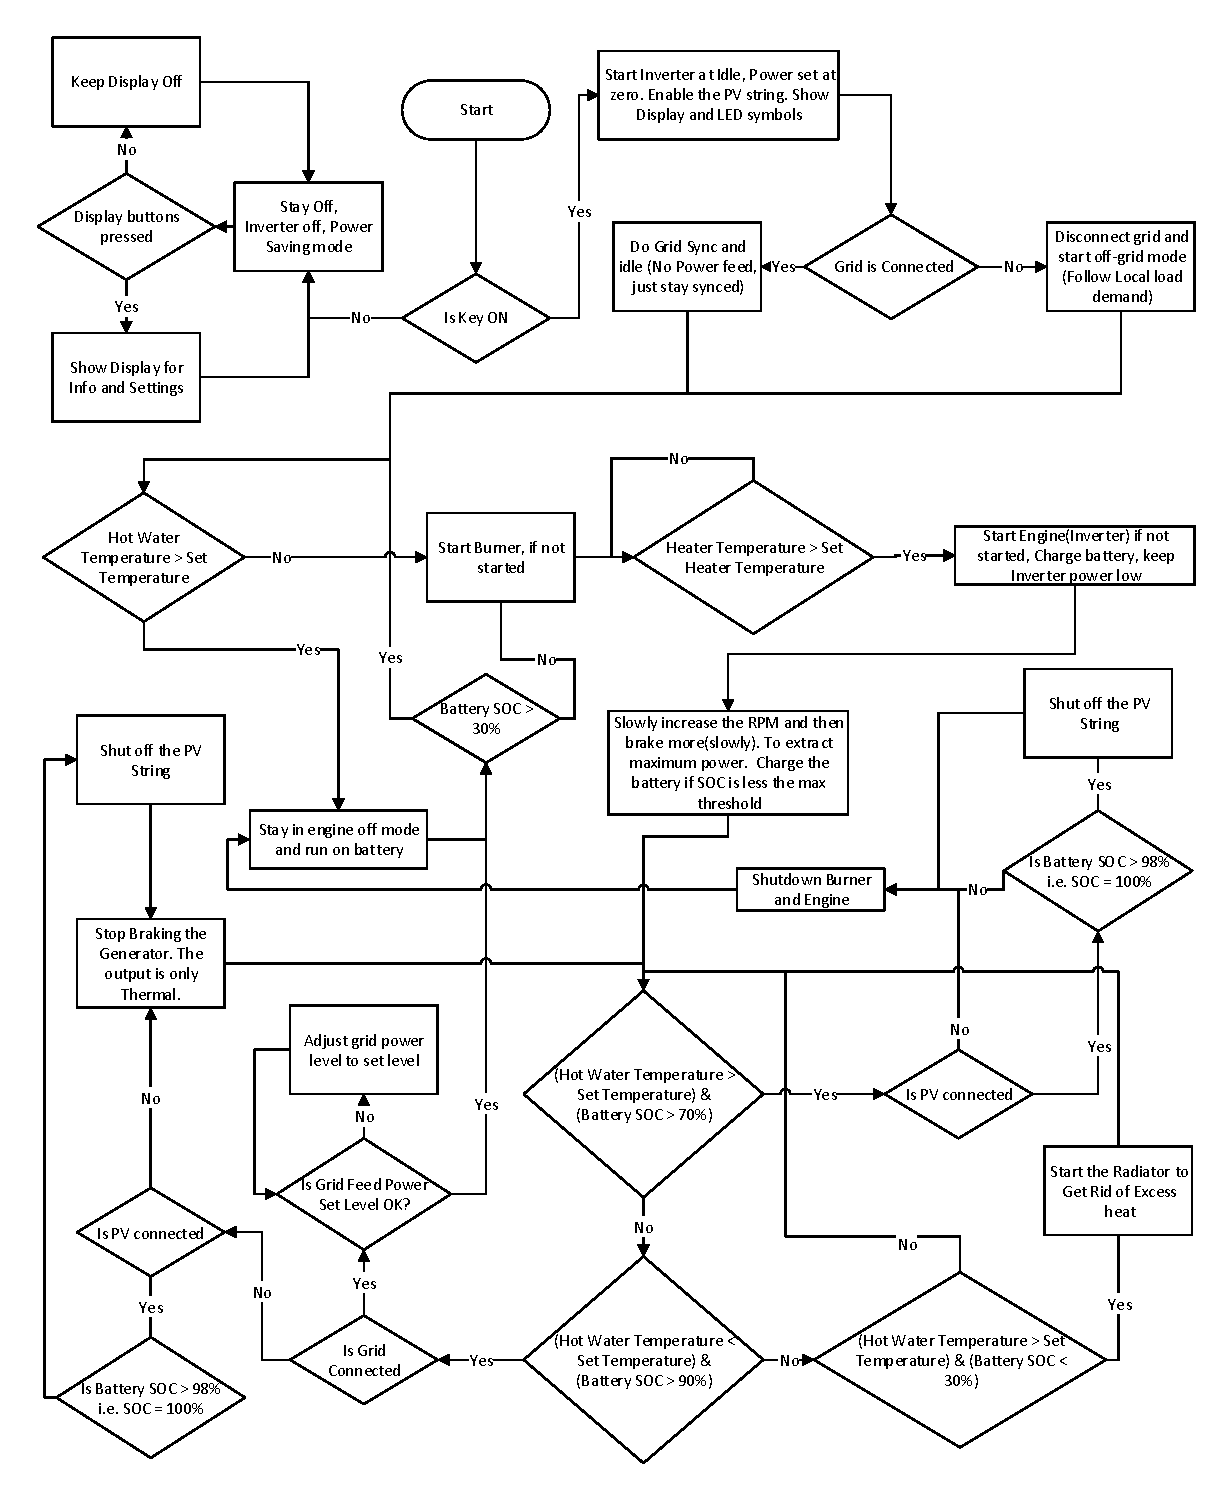
\includepdf[scale=0.60, pagecommand={\thispagestyle{fancy}}]{portable/Portable_Flowchart.pdf}
%\caption{Operation flow in portable system.}
\vspace*{6in}
\captionof{figure}{Operation flow in portable system.}\label{fig: Operation flow in portable system.}
\end{figure}
\newpage

\clearpage
\newpage
\begin{figure}
	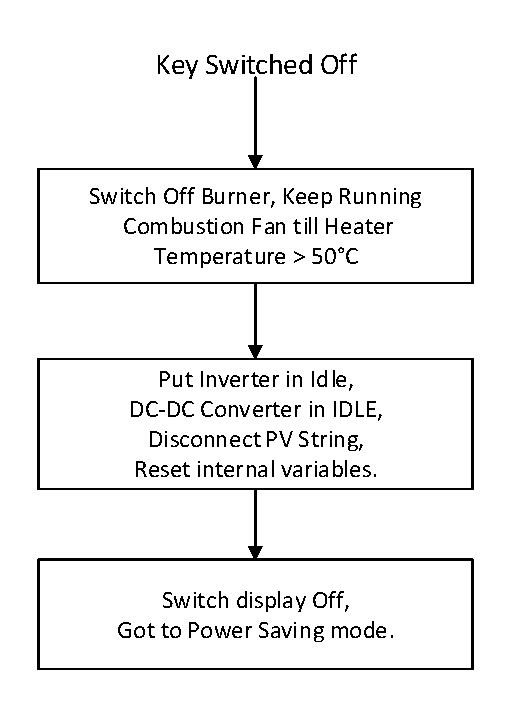
\includepdf[scale=0.60, pagecommand={\thispagestyle{fancy}}]{portable/KeyOff_Sequence.pdf}
\vspace*{7in}
\captionof{figure}{Key Switch Off sequence in portable system.}\label{fig: Key Switch Off sequence in portable.}	
\end{figure}

\clearpage
\subsection{External thermostat}
\label{ch:extthermostat}
If external thermostat function is disabled, the key functionality(ON/OFF) works as usual. Otherwise, the external thermostat works in conjunction with the key. If the key is OFF, the portable will always be OFF.
If the key is ON and thermostat function is enabled, the engine will start when external temperature sensor drops below the lower threshold.
And, the portable will switch OFF, when the temperature sensor exceeds the higher threshold value. Flowchart of external thermostat functionality is shown in \figref{ExternalThermostatSequence}.

\begin{figure}[h]		
	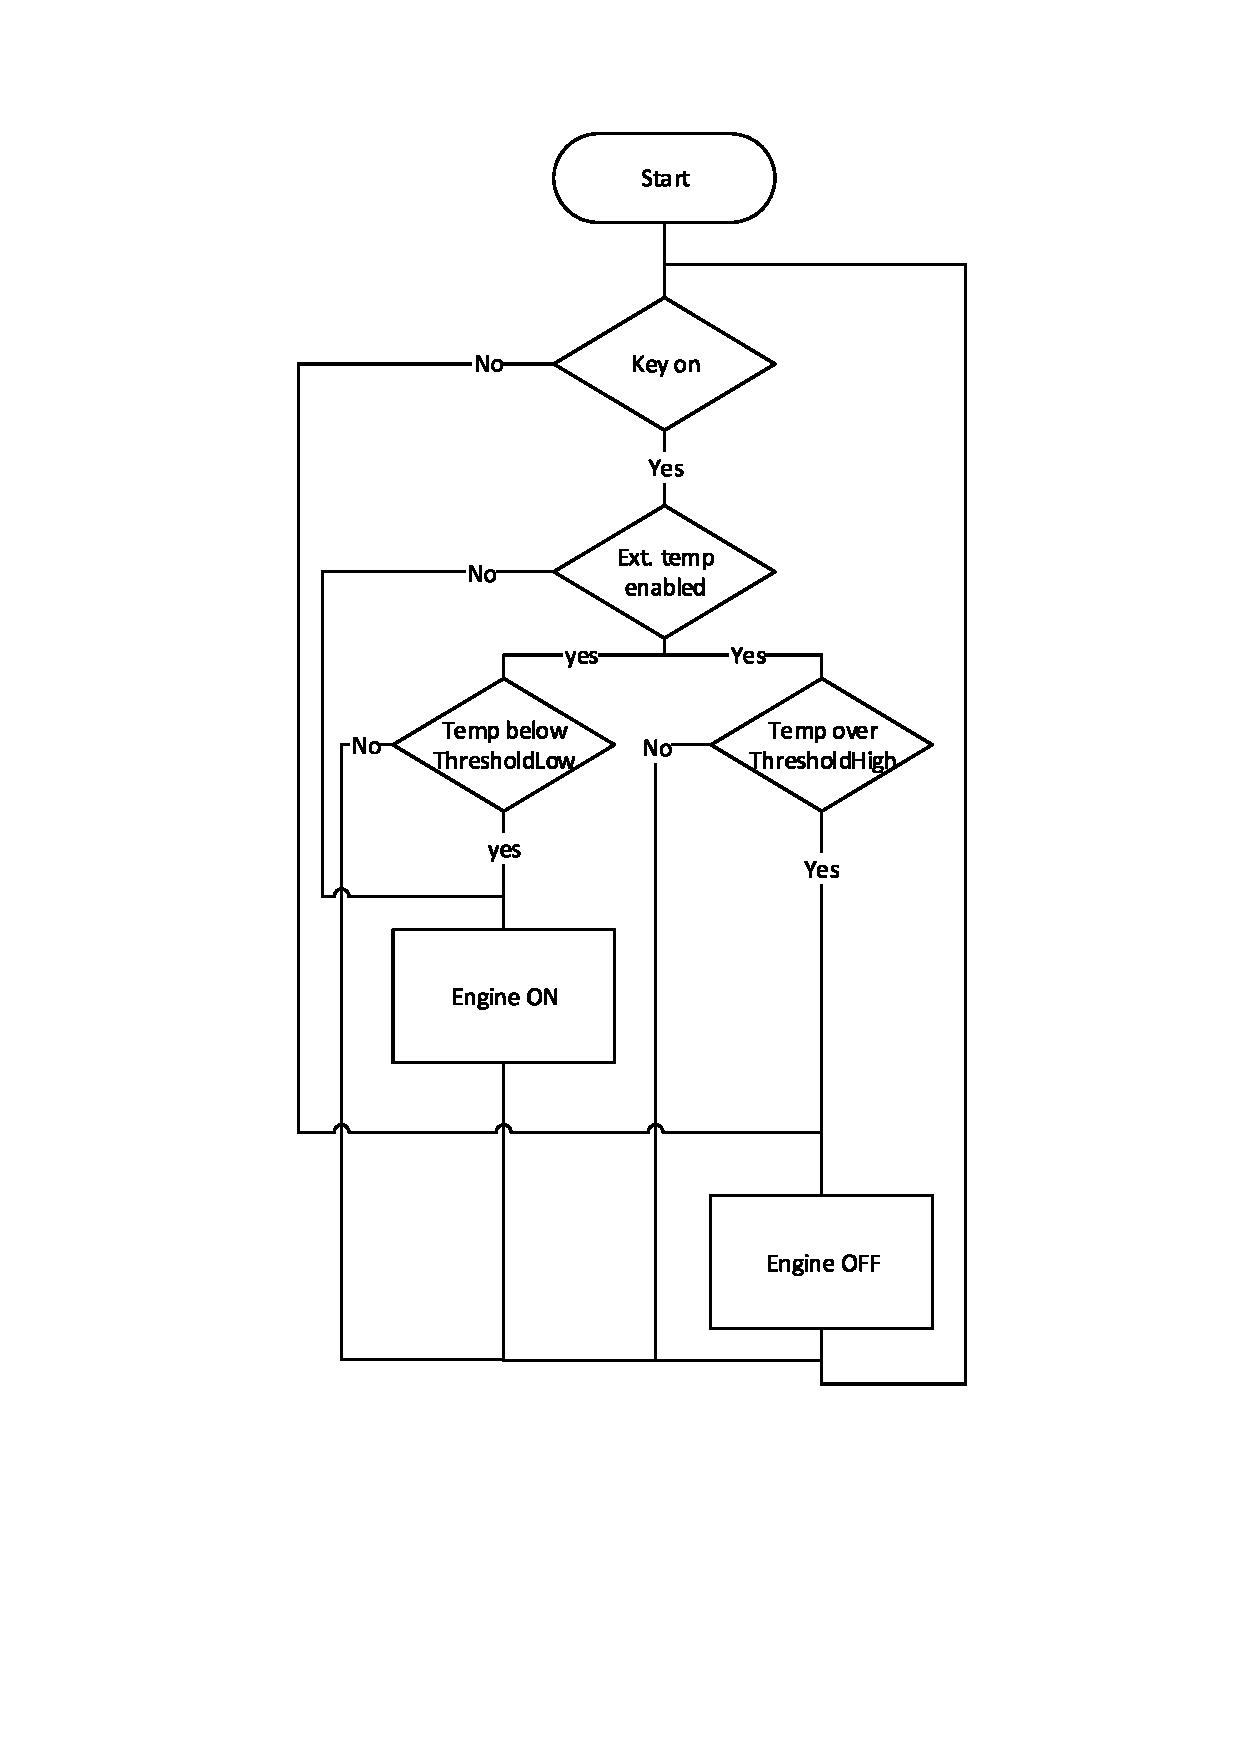
\includepdf[scale=0.4, pagecommand={\thispagestyle{fancy}}]{portable/ExtTempSensor.pdf}
	\vspace*{3.8in}
	\captionof{figure}{External thermostat sequence in portable system.}\label{fig:ExternalThermostatSequence}	
\end{figure}


